\chapter*{Rules}
\section*{Designing Rules for a VR Environment}

To ensure realism and to estimate functionality of the virtual reality simulation a set of rules for the system should be drawn. The core rules can be separated into three primary groups; the system, the users, and the virtual equipment. However, these rules are set prior to implementation but are based on observations made in the training room as well as interviews with Jane Petersson. The mindmap of these rules is shown in Figure  \autoref{fig:Rules}.

\begin{figure}[H]
\centering
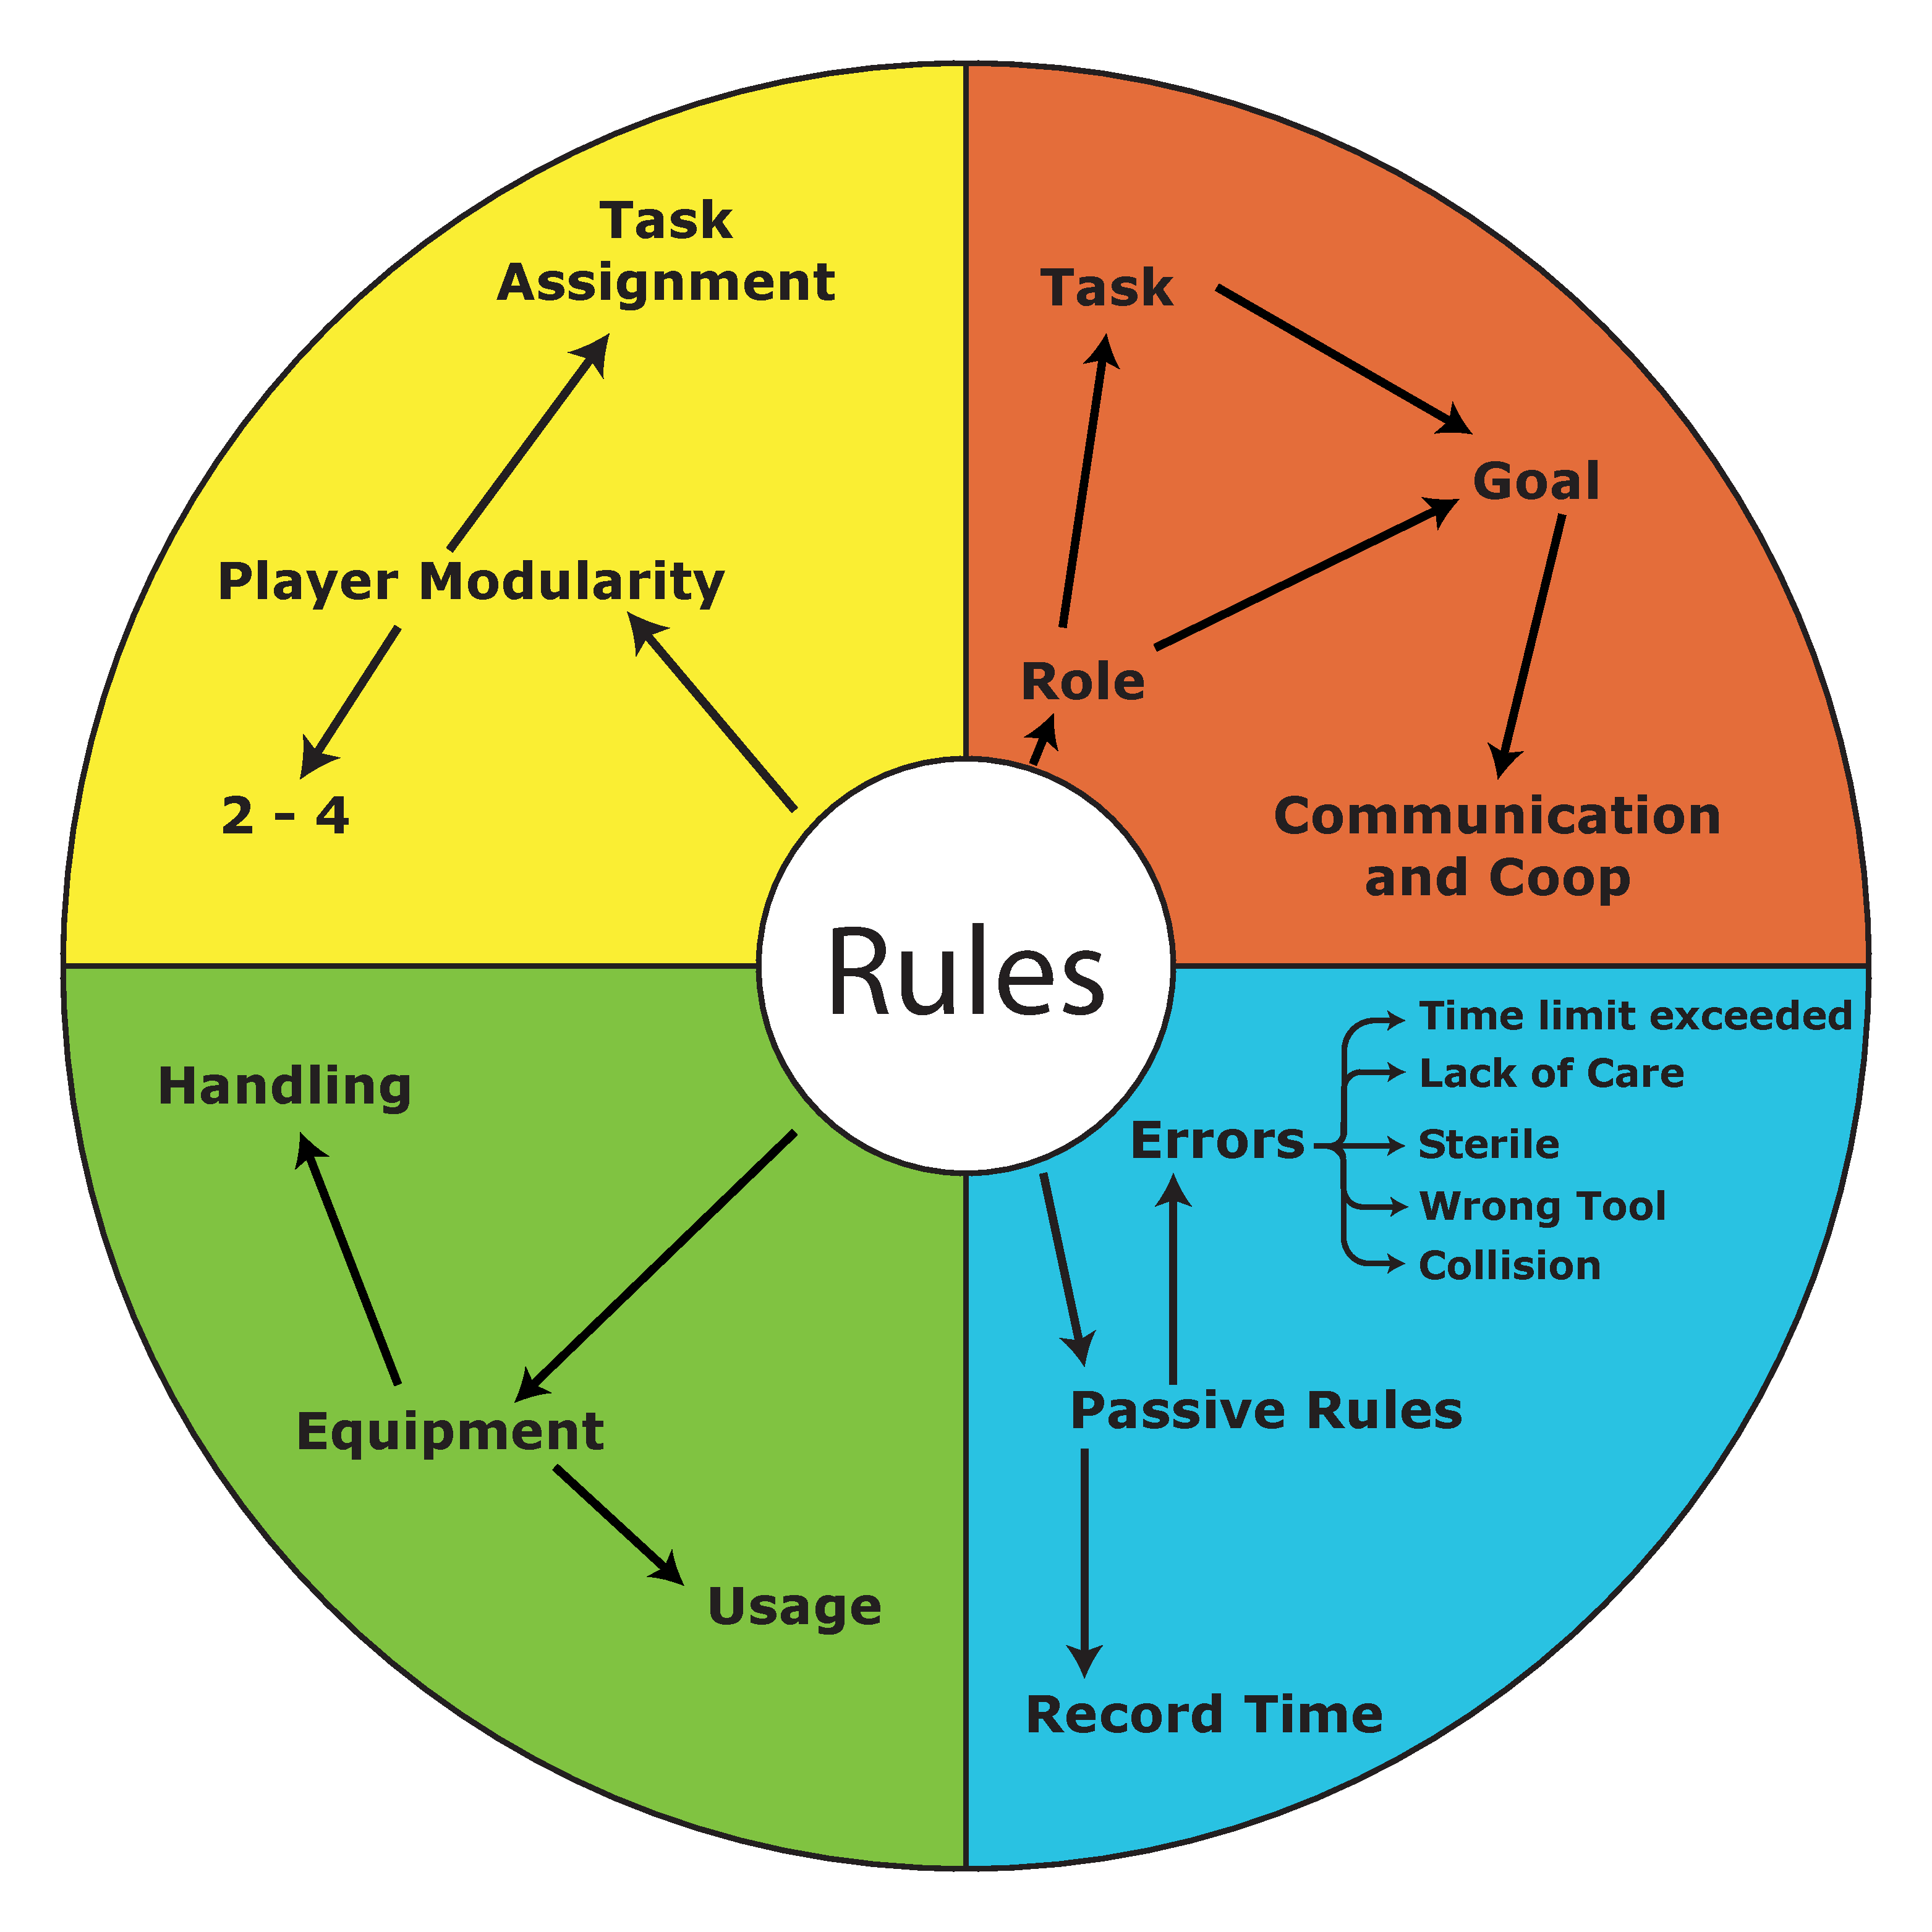
\includegraphics[width=0.65\textwidth]{WorksheetRules/brainstorm_rules}
\caption{Mindmap}
\label{fig:Rules}
\end{figure}

\subsection*{The System}
The rules set for the system can be considered passive. These rules primarily exist to accurately recreate the environment and ensure the proper functionality of the surgical equipment. These rules also track any errors that might be done by the users, such as poor positioning of the robot arms or incorrect tool placement.

\subsection*{The User}
The users in the scene should be designated a specific role which entails different tasks, but they should not be limited by that role. Completing a task as a group, rather than multiple individuals should be the primary focus for the users, since communication is vital to the success of the simulation.

\subsection*{The Equipment}
The equipment's rules should primarily focus on their specific use and how they should be handled by the users. Furthermore it should also include how the equipment should respond to certain user actions or other objects within the scene.
